\chapter*{Введение}
\addcontentsline{toc}{chapter}{Введение}


Параллельные вычисления - способ организации компьютерных вычислений,
при котором программы разрабатываются как набор взаимодействующих вычислительных процессов, работающих параллельно (одновременно).
\\


\textbf{Целью работы:} изучение параллельных вычисления,
работая с разреженными матричными структурами.
\\

\textbf{Задача:}
Реализовать в параллельном режиме поиск строки с максимальной суммой элементов в симметричной разреженной матрице в схеме Дженнингса (см. ТСД). Матрицу не распаковывать.



\chapter{Аналитический раздел}
\label{cha:analysis}

% В данном разделе будет приведено описание алгоритмов и модель
% вычислений для оценок трудоемкости.

% дать постановку задачи, описать решение, привести тесты и примеры работы, интерпретировать результаты.

\section{Симметричная разреженная матрица в схеме Дженнингса}

Дженнингс [Jennings, 1966] предложил эффективную схему хранения
симметричных матриц, и она вследствие своей простоты стала
весьма популярной. Называется она профильной схемой, или
схемой переменной ленты.
Для каждой строки i симметричной матрицы А положим

$\beta_i = i - j_{min}(i)$

где $j_{min}(i)$ - минимальный столбцовый индекс строки i,
для которого $a_{ij} \ne 0$.


\begin{figure}[h!]
    \centering
    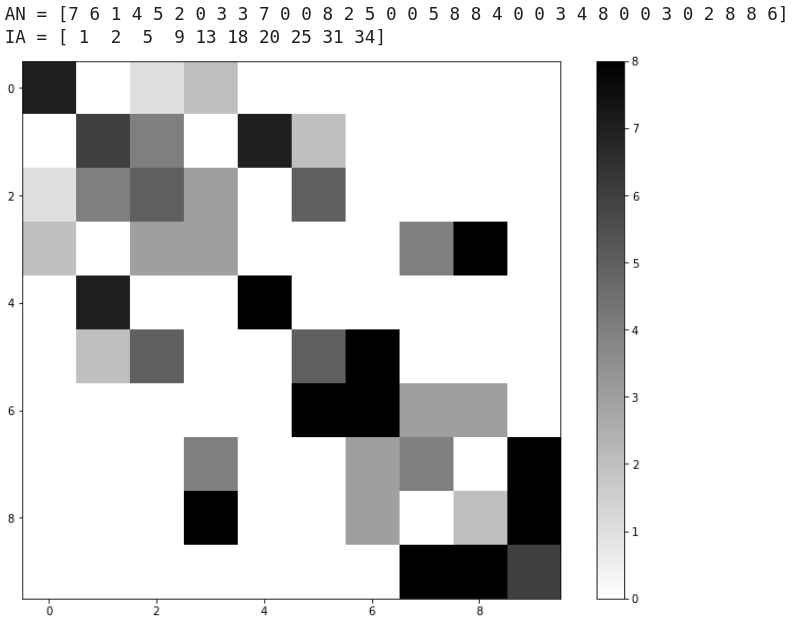
\includegraphics[width=0.8\textwidth]{inc/p1.png}
    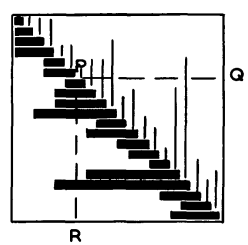
\includegraphics[width=0.32\textwidth]{inc/p2.png}
    \caption{Схема Дженнингса}
\end{figure}



\chapter{Конструкторский раздел}
\label{cha:design}

В данном разделе будет приведено описание алгоритмы,
который суммирует элементы в строке без распаковки матрицы.

\section{Вычисление суммы строк матрицы в схеме Дженнингса}

На рисунках \ref{fig:2.2} показаны пути, по которым вычисляется сумма строки матрицы.



\begin{figure}[h!]
    \centering
    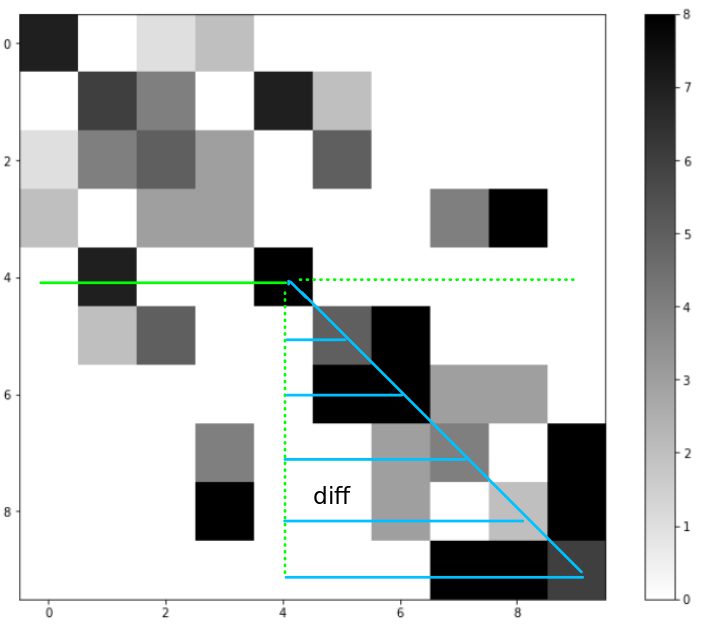
\includegraphics[width=0.8\textwidth]{inc/p3.png}
    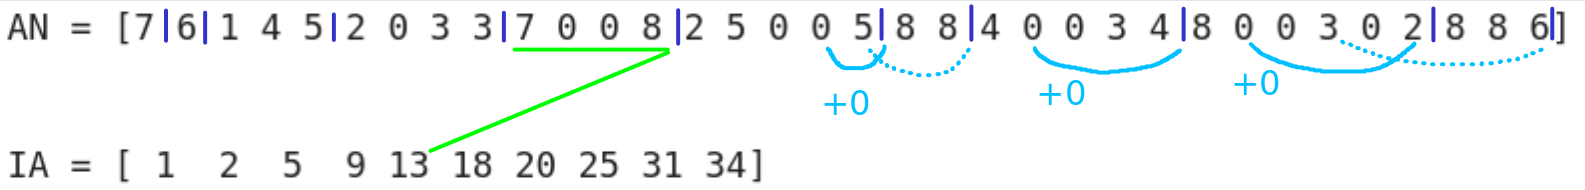
\includegraphics[width=1\textwidth]{inc/p4.png}
    \caption{Вычисление суммы строк матрицы в схеме Дженнингса}
    \label{fig:2.2}
\end{figure}


\pagebreak
\subsection*{Код}

\begin{lstlisting}[language=c++]
int sum_row(int n)
{
    int start = (n == 0) ? 0 : IA[n-1];
    int stop = IA[n];
    int sum = 0;

    for (int i = start; i < stop; i++)
        sum += AN[i];

    for (int i = n+1, diff = 2; i < N; i++, diff++)
        if (IA[i] - IA[i-1] >= diff)
            sum += AN[IA[i]-diff];

    return sum;
}
\end{lstlisting}


\section{Многопоточная реализация обхода строк матрицы}

Реализация многопоточности просто разбивается на n меньших областей и находит индекс и максимальную сумму в этой области. Затем найти индекс строки с максимальной суммой из n областей.


\chapter{Технологический раздел}
\label{cha:impl}


\section{Средства реализации}

Язык программирования: C++, Python

Библиотеки: matplotlib, scipy.sparse
(python, для генерации случайных матриц и визуализации)

Редактор: VS Code

Я использую эти инструменты потому, что они мощные, широко используемые.



\section{Листинг кода}

\lstinputlisting[
    language=c++,linerange={0-180},
    caption=Шаблон разреженной матрицы
    ]{inc/code.h}

\vspace{1cm}

\lstinputlisting[
    language=python,linerange={0-100},
    caption={Функции поддерживают создание данных, построение графиков, экспорт в тестовые файлы}
    ]{inc/code2.py}




\chapter{Экспериментальный раздел}
\label{cha:research}

В данном разделе будет приведено пример работы программы,
результаты тестирования и сравнение времени работы
последовательного и параллельного алгоритма Винограда.

\section{Пример работы и результаты тестирования}
На рисунке \ref{fig:4.1} и \ref{fig:4.2} приведен пример работы программы и результат теста.

\begin{figure}[h]
    \centering
    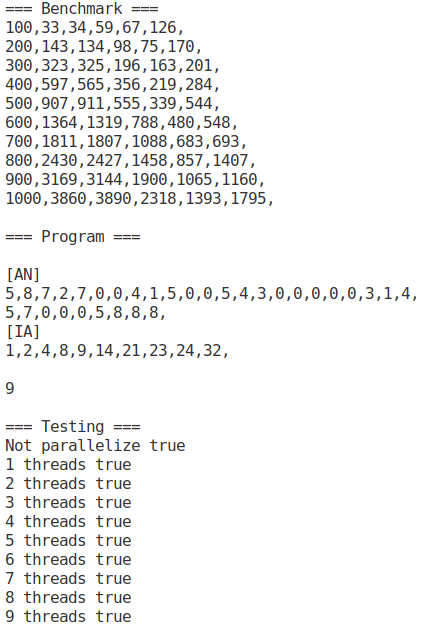
\includegraphics[width=0.6\textwidth]{inc/e1.png}
    \caption{Пример работы и результаты тестирования}
    \label{fig:4.1}
\end{figure}

\begin{figure}[h]
    \centering
    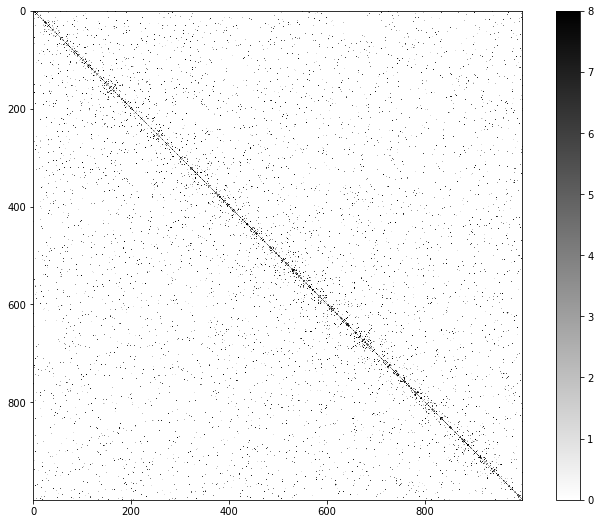
\includegraphics[width=0.48\textwidth]{inc/m1.png}
    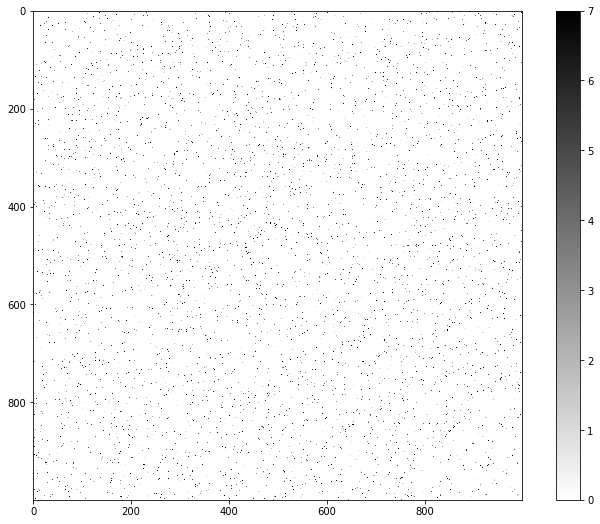
\includegraphics[width=0.48\textwidth]{inc/m2.png}
    \caption{Пример сгенерированной матрицы (1000x1000)}
    \label{fig:4.2}
\end{figure}



% На рисунке \ref{fig:4.2} приведен  с использованием фреймворка google test.

% \begin{figure}[h]
%     \centering
%     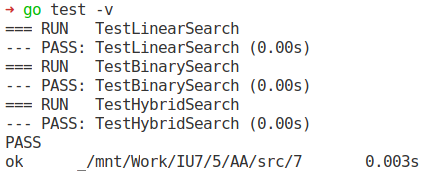
\includegraphics[width=0.6\textwidth]{inc/test.png}
%     \caption{Результаты тестирования}
%     \label{fig:4.2}
% \end{figure}


\pagebreak
\section{Сравнение времени работы}

Операционная система - Ubuntu 20.04.1 LTS

Процессор - Intel® CoreTM i5-7300HQ CPU @ 2.50GHz × 4 (ЦП 4 ядра 4 потока)

В таблице \ref{tabular:benchmark} приведены замеры времени работы.



\def\arraystretch{1.2}
\setlength\tabcolsep{0.4cm}

\begin{table}[h]
    \centering
    \csvreader[tabular=|c|c|c|c|c|c|,
        table head=\hline
        \bfseries Размер
        & \bfseries Последо.
        & \bfseries 1 поток
        & \bfseries 2 поток
        & \bfseries 4 поток
        & \bfseries 8 поток
        \\\hline,
        late after line=\\\hline]
        {inc/benchmark.csv}{}
    { \csvcoli & \csvcolii & \csvcoliii & \csvcoliv & \csvcolv & \csvcolvi}
    \caption{\label{tabular:benchmark} Времени работы ($10^{-6}$с)}
\end{table}



\clearpage
\begin{figure}[!h]
    \centering
    \begin{tikzpicture}
        \begin{axis}[
            scale=2,
            axis lines=left,
            xlabel=Размер матрицы,
            ylabel={Время, $10^{-6}$с},
            legend pos=north west,
            xmajorgrids=true,
            ymajorgrids=true
        ]
            \addplot table[x=n,y=t0,col sep=comma] {inc/benchmark.csv};
            \addplot table[x=n,y=t1,col sep=comma] {inc/benchmark.csv};
            \addplot table[x=n,y=t2,col sep=comma] {inc/benchmark.csv};
            \addplot table[x=n,y=t4,col sep=comma] {inc/benchmark.csv};
            \addplot table[x=n,y=t8,col sep=comma] {inc/benchmark.csv};
            \legend{Последовательный, 1 поток, 2 поток, 4 поток, 8 поток}
        \end{axis}
    \end{tikzpicture}
    \caption{Зависимость времени работы алгоритмов умножения матриц от размеры матрицы и количество потоков}
    \label{fig:4.4}
\end{figure}


% % \section{Сравнительный анализ на материале экспериментальных данных}
% % эксперименты+выводы

\section{Вывод}

График показывает, что многопоточная версия более эффективна,
когда количество потоков увеличивается, производительность увеличивается с увеличением количества потоков до тех пор,
пока она не станет равной количеству ядер процессора, и наиболее эффективна,
когда количество потоков равно количеству ядер процессора.
Затем, если количество потоков увеличивается, происходит небольшое уменьшение
из-за необходимости управлять большим количеством потоков.



\chapter*{Заключение}
\addcontentsline{toc}{chapter}{Заключение}

В ходе работы было изучено параллельных вычисления,
работая с разреженными матричными структурами.
Было сравнить временные характеристики последовательного и параллельного реализации
и сделаны следующие выводы:

\begin{itemize}
    \item производительность увеличивается с увеличением количества потоков до тех пор,
    пока она не станет равной количеству ядер процессора;
    \item многопоточная версия наиболее эффективна когда количество потоков равно количеству ядер процессора;
    \item время выполнения с использованием 4 потоков всего 46.5\% по сравнению с последовательным выполнением (на матрице 1000x1000).
\end{itemize}
